\documentclass{article}[12pt,letterpaper]
\usepackage[T1]{fontenc}
\usepackage{mathptmx}
\usepackage[utf8]{inputenc}
\usepackage[margin=1.00in]{geometry}
\usepackage{xspace}
\usepackage{bigfoot}
\usepackage{pgfplots}
\pgfplotsset{compat=1.15}
\usepackage{tikz}
\usetikzlibrary{shapes.geometric, arrows}
\usepackage{pbox}
\usepackage[authordate,bibencoding=auto,strict,backend=bibtex,natbib]{biblatex-chicago}
\addbibresource{walking.bib}
\usepackage{caption}
\captionsetup{skip=0pt}
\usepackage{setspace}
\usepackage{graphicx}
\onehalfspacing

\tikzstyle{startstop} = [rectangle, rounded corners, minimum width=3cm, minimum height=1cm,text centered, draw=black, fill=gray!30]
\tikzstyle{io} = [trapezium, trapezium left angle=70, trapezium right angle=110, minimum width=3cm, minimum height=1cm, text centered, draw=black, fill=blue!30]
\tikzstyle{process} = [rectangle, minimum width=3cm, minimum height=1cm, text centered, draw=black, fill=blue!30]
\tikzstyle{decision} = [rectangle, rounded corners, minimum width=3cm, minimum height=1cm,text centered, draw=black, fill=yellow!30]
\tikzstyle{arrow} = [thick,->,>=stealth]

\begin{document}
\newcommand{\cadi}{CO\textsubscript{2}\xspace}
\newcommand{\methane}{CH\textsubscript{4}\xspace}
\pagenumbering{gobble}

\title{Is Walking ``Greener'' Than Driving? It depends on Your Diet!}
\date{\today}
\author{Mico Mrkaic\thanks{I thank Sebastian Acevedo, Nicoletta Battini, Stephan Danninger, Selim Elekdag, Eve Errickson, Anna Ilyina, Vladimir Klyuev, Subir Lall, Natalija Novta, Holger Sieg, and Petia Topalova for their comments. Special gratitude goes to Aljo\v{s}a Feldin, who verified some key numbers in the paper and saved me from embarrassing mistakes. All remaining errors are my own.}
\\International Monetary Fund\\Washington DC, 20031, USA\\email: mmrkaic@imf.org.}

\maketitle
\begin{abstract}\noindent Climate change mitigation and adaptation require changes to our overall lifestyle, including what we eat and how we travel. It appears to be an obvious truth that walking, running, or cycling instead of driving dramatically reduces the emission of greenhouse gasses (GHG). However, eating a diet rich in foods of animal origin has been shown to drastically reduce environmental benefits of cycling. I advance the existing literature of the benefits human powered transportation in four ways. First, by using accurate measures of energy expenditure in cycling instead of customary crude estimates. Second, I extend the analysis to environmental benefits to walking and running. Third, I use comprehensive measurements of GHGs in food production, including \methane, to assess the full environmental impact of human powered transport. Finally, I compare the GHG impact of human powered transportation to that of driving and flying using realistic data on diets for a select group of countries. To maximize the benefits of human powered transport, I suggest imposing excise taxes on meat and other animal products with concommitant measures to assist the low income househyolds, and eliminating direct and indirect subsidies of animal sourced foods.
\end{abstract}

\newpage
\pagenumbering{arabic}
\section{Introduction}
% https://archive.curbed.com/2017/4/18/15333796/best-cities-bike-commute-us-cycling
Climate change mitigation and adaptation require changes to our overall lifestyle, including what we eat and how we travel. Consequently, many cities and countries have recently invested in infrastructure to support cycling and walking with the goal of improving public health and the environment. The United Kingdom has recently committed to invest 2 billion pounds in walking and cycling projects and France has a plan to spend two billion euros to improve cycling infrastructure. In 2020 Washington DC embarked on a plan to build 20 miles of new protected bike lanes over 3 years. Similar plans are in motion in many other jurisdictions.

The benefits of walking, cycling and running as modes of transport are numerous and well documented. Physical activity improves health. Fewer cars on the roads, especially older models, reduce local pollution and traffic congestion. These benefits are subject of numerous studies and are not discussed here. The issue I address in this paper is an often implied claim that discarding automobiles and other internal combustion vehicles in favor of human powered transportation necessarily and unconditionally helps fight climate change. Since no fossil fuels are burned while walking or cycling as opposed to driving, emissions of greenhouse gasses (GHGs), most important of which are carbon dioxide (\cadi) and methane (\methane), should be reduced.\footnote{While some GHGs in the atmosphere are essential for life, their recent growth is excessive.} 

However, the reality is more nuanced. While it is true that automobiles burn fossil fuels and generate GHGs, so does the production of food. When we walk, run or cycle, we use energy stored in food and {\em indirectly} emit GHGs. For this reason, we must account for the emissions of GHGs due to human generation of mechanical power and optimize diets to maximize environmental benefits of human powered transportation. The goal of this paper is to use advances in bicycle technology, physiological and metabolic calculations as well as improvements in the estimation of GHG emissions of food production to provide precise estimates of the GHG impact of walking, running and cycling for a select group of countries. Based on the comparison of these emission to those from automobiles and airplanes I make some modest proposals.

\subsection{A Surprising Example}
To motivate the general discussion, consider my leisurely bicycle commute to work as an illustrative example. Cycling is ideally suited to illustrate the issue, because mechanical power that is produced by the rider, can be measured accurately every second with modern power meters. Cycling computers add these measurements and calculate total mechanical work performed during a ride. My 27 kilometers long ride to work took me 1 hour and 24 minutes. With average power of 104 Watts I performed 520 kJ of mechanical work.\footnote{Mechanical work was measured using a Quarq DZero power meter with the precision of about 1-2 percent.}

If we know how efficiently cyclists convert energy in food into mechanical work, we can calculate caloric requirements of cycling. Substantial recent research on the efficiency of cycling, for example \citet{delta-cyc-1}, \citet{cycling-efficiency-review} and \citet{efficiency-young-old}, have shown that cyclists are about 25\% efficient at generating mechanical work---they have to consume four Joules of energy in food to produce one Joule of mechanical work. Consequently, my ride burned 2.1 MJ or 500 Calories.\footnote{``Big C'' Calorie is also known as kilo-calorie (kcal) and equals 4,184 Joules.} At the same effort level, I would burn about 1,850 Calories to bike 100 kilometers.

One final question remains. How do we get from 1,850 worth of food Calories to GHG emissions? We need to look at the amount of \cadi and its equivalents that are generated in food production. Figure \ref{fig:table-ghg-per-1000-calories} shows the GHG equivalents of select foods per 1000 calories.\footnote{For the source see \citet{carbon-footprint-food-methane}.}
If I fueled my ride with beef, I would generate 36.4 kg of \cadi equivalents for every 1000 calories, or 67.5 kg per 1,850 calories. As Figure \ref{fig:GHG-and-means-of-transportation} shows, this would greatly exceed GHG emissions from driving a car and even the emissions from a long-haul first class flight. Eating beef is a true environmental luxury! Avoiding meat is not necessarily green---if I fueled my ride with cheese, the \cadi equivalent would be 11.4 kg---better than driving an midsize car, but worse than sharing a car ride. Eating plants improves the picture dramatically. My ride, fueled with rice, would generate 2.2 kg of \cadi equivalent, while eating potatoes would reduce the emissions to only 1.2 kg. We see that cycling is not unconditionally better for the climate change. If ardent beef eaters abandon their cars in favor of cycling, they might actually harm the environment.

It should be emphasized that some dietary options in the example are extreme and that fueling human powered transportation with actual---real world---diets would likely lead to smaller environmental impacts. For this reason, I analyze below the GHG impact that is based on realistic diets for a select set of countries.

\subsection{Improving Upon Existing Literature}
Evaluation of the GHG impact of human powered transport is not a new endeavor, but it has been mostly limited to cycling. The first analysis is \citet{berners-lee-2010}, who estimated the diet-dependent GHG impact of cycling and, somewhat provocatively, concluded ``Two people cycling along using energy from cheeseburgers is equivalent to those same people sharing a ride in an efficient car.``
More favorable to cycling is the analysis by the European cycling Federation \citet{ecf2011}. However, the analysis assumes a very low value for energy expenditure of cycling and neglects the impact of \methane that is generated in food production. Finally, \citet{thorpe-keith_2016} find that ``biking has a surprisingly similar marginal impact to driving on a per kilometer basis, and depending on your diet can cause similar greenhouse gas emissions and more land use.'' His analysis relies on a rough estimate of cycling energy expenditure, which weakens its conclusions.
% www.bikeradar.com/features/long-reads/cycling-environmental-impact/
%https://biofriendlyplanet.com/green-alternatives/transportation/environmental-reasons-to-start-riding-your-bicycle-more/

This paper expands upon this literature in four ways. First, it uses accurately calculated cycling power values instead of guesses or crude estimates. Second, it extends the analysis to walking and running using accurate metabolic formulas. Third, it comprehensively accounts for \cadi equivalents in food production, including \methane, to obtain the full environmental impact of human powered transport. Finally it compares the GHG impact of human powered transportation to that of driving and flying using realistic data on diets for a select group of countries and proposes some modest policies. Finally, \citet{Mizdrak2020} quantify the effects of human powered locomotion for cycling and walking, but their estimates of cycling power are based on metabolic formulas and not on physics.

\section{GHG Emissions and Internal Combustion Engines}
%% What I find interesting is that this study highlights the importance of looking at the consumption side, not just the production side, which is what you are focusing on in your paper.  
To generate mechanical work, internal combustion engines burn carbohydrates and release exhaust gases, including \cadi, water vapor and others. Some of these gases, primarily \cadi, trap infrared radiation in the atmosphere and contribute to global warming. The intensity with which vehicles emit GHGs is measured in kilograms of \cadi equivalents per unit distance. In this paper I quote this intensity in kilograms of \cadi equivalents per 100 kilometers. Table \ref{fig:GHG-and-means-of-transportation} shows GHG emissions for some representative modes of transportation.\footnote{The amount of GHG released in the production in fossil fuels is typically small, on the order of magnitude of a percent of the amount released in burning the fuels, as shown in \citet{yeh2017}. It follows that, at least for the purpose of this paper, we can equate the amount of GHG released in the burning of fossil fuels in engines with the total amount of GHG associated with the fossil fuels.}

\begin{figure}
  \centering
  \caption{GHG emissions per passenger, \cadi equivalent in kg per 100 km. (Source: \cite{greenhouse-gas-reporting-conversion-factors-2019} and \cite{travel-carbon-footprint}.)}
  \label{fig:GHG-and-means-of-transportation}
  \includegraphics[scale=0.5]{fig_1.png}
\end{figure}

Some patters readily emerge from the table. First, fossil fuel powered cars predictably emit more GHGs than their electric equivalents, but electric cars are not zero carbon machines.\footnote{The GHG emissions of electric vehicles depend on the technology of electricity production. In general, electric vehicles are substantially cleaner than standard vehicles. A UK car is used as a benchmark. See \citet{holland2016} for a deeper discussion.} Second, ride sharing drastically reduces carbon footprint. Sharing rides in electric vehicles could be particularly effective. Third, long haul first class flights (where passengers use more space on the plane) are highly polluting and serve as a benchmark of high emissions---something that will be explored below. And finally, railway transport is comparatively clean.\footnote{The analysis includes only direct GHG emissions of driving, not the indirect emissions associated with producing the vehicle.}

\section{GHG and Human Powered Transport}
It might appear that human powered transport does not contribute to GHG emissions, since no fossil fuels are burned when muscles provide locomotive power. A deeper insight quickly dispels this notion. Fossil fuels are burned and \methane is released in food production. Since energy cannot be created out of nothing, mechanical work must be fueled by food. It follows that humans indirectly generate GHGs when they perform mechanical work.

It is important to note that conservation of energy requires humans to increase their food intake when they increase their physical activity---at least in the long run. If people increased their physical activity without increasing their food intake, they would lose weight in the short to medium run. However, this is not sustainable. If they persisted without increasing their caloric intake, they would inevitably starve, continue losing weight and get sick. \footnote{Only minute amounts of additional work can be sustained if food intake is not increased due to lower resting energy requirements after weight loss. A calculation in the Appendix shows why eating extra food is necessary.} \footnote{People might reduce their exercise volume when walking instead of driving. However, to achieve environmental sustainability, the GHG emissions due to human physical activity still need to be minimized by the appropriate dietary choices, as will be shown below.}

It is important to clarify the role of direct \cadi emissions (i.e. breathing) by humans. The \cadi breathed out by humans (and other living creatures) has a net zero contribution to GHG emissions. If the contribution were not zero, the Earth would have experienced a global warming catastrophe in the distant past due to the volume of \cadi emitted in the past by breathing organisms. What matters for GHG emissions generated by human powered transportation is the source of food used to fuel these activities, the amount of fossil fuels used in the production of the food and the amount of other GHGs foods release during their production. Living creatures who feed on naturally grown foods do not contribute to net GHG emissions, because they are a part of a closed system.

To quantify GHG emissions due to human mechanical work, I proceed in two steps. First, I estimate the energy needed by a US person of average size and weight to run, walk or cycle 100 kilometers on flat terrain. Second, I multiply these energy requirements with GHG emissions of various foods per Calorie to obtain the total GHG emissions for walking, running and cycling.\footnote{Three typical cycling profiles---slow, moderate and fast---are included in the table.}

\subsection{Caloric Requirements of Walking, Running and Cycling}
Calculating accurate caloric requirements of walking, running and cycling is crucial to obtain their GHG impact. The details of the calculations are in the Appendix, here we present only an overview. Walking and running calories are calculated as multipliers ---metabolic equivalents or METs---of the resting metabolic rate (RMR). The resting metabolic rate depends on the size, age and gender of the person. The most accurate method to determine the RMR is laboratory measurement. However, accurate formulas that give estimates of the RMR also exist and are used in this paper. The METs depends on the type of the activity. For walking and running they are determined by the speed with which a person moves and the slope of the terrain.

Caloric requirements of cycling are calculated differently. Cycling power is described accurately with a simple mechanical formula. It depends on the size of the rider and the linear and cubic terms of the speed, accounting for rolling and aerodynamic resistance, respectively. Power is converted into caloric requirements by taking into account the efficiency with which the human body generates mechanical power when cycling. A summary of calculations of caloric requirements for walking, running and cycling is graphically presented in Figure \ref{fig:kcal-per-100-km}.

The results of the calculations are summarized in Figure \ref{fig:table_METs_walk_run}, which shows the caloric requirements to run, walk or cycle 100 kilometers. The calculations are for the ``average US human''---the  average of the average man and woman respectively.\footnote{For the source of average body measurements see \cite{body-measurements}.}

\begin{figure}
\centering
\caption{Calculating caloric requirements of cycling, walking and running}
\label{fig:kcal-per-100-km}
    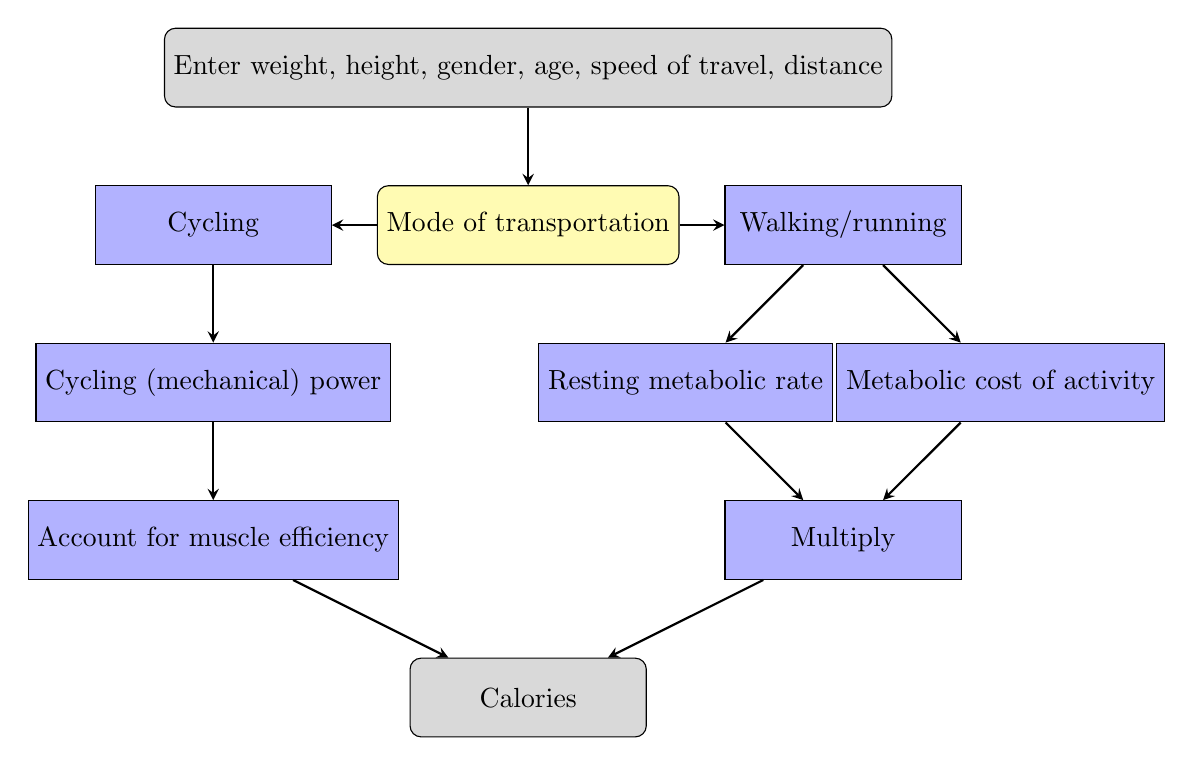
\begin{tikzpicture}[node distance=2cm]
    \node (pro1) [startstop] {Enter weight, height, gender, age, speed of travel, distance};
    \node (dec1) [decision, below of=pro1] {Mode of transportation};
    \node (pro2a) [process, left of=dec1, xshift=-2cm] {Cycling};
    \node (cyc1) [process, below of=pro2a, xshift=0cm] {Cycling (mechanical) power};
    \node (cyc2) [process, below of=cyc1, xshift=0cm] {Account for muscle efficiency};
    \node (cyc3) [startstop, below of=cyc2, xshift=+4cm] {Calories};
    \node (pro2b) [process, right of=dec1, xshift=2cm] {Walking/running};
    \node (wr1) [process, below of=pro2b, xshift=-2cm] {Resting metabolic rate};
    \node (wr2) [process, below of=pro2b, xshift=+2cm] {Metabolic cost of activity};
    \node (wr3) [process, below of=wr1, xshift=+2cm] {Multiply};
    \draw [arrow] (pro1) -- (dec1);
    \draw [arrow] (dec1) -- (pro2a);
    \draw [arrow] (pro2a) -- (cyc1);
    \draw [arrow] (cyc1) -- (cyc2);
    \draw [arrow] (cyc2) -- (cyc3);
    \draw [arrow] (dec1) -- (pro2b);
    \draw [arrow] (pro2b) -- (wr1);
    \draw [arrow] (pro2b) -- (wr2);
    \draw [arrow] (wr2) -- (wr3);
    \draw [arrow] (wr1) -- (wr3);
    \draw [arrow] (wr3) -- (cyc3);
    \end{tikzpicture}
\end{figure}

\begin{figure}
  \centering
  \caption{Food intake in Calories needed to move 100 kilometers on flat terrain. (Source: author's calculations.)}
  \label{fig:table_METs_walk_run}
  \includegraphics[scale=0.5]{fig_2.png}
\end{figure}

In running and walking, expended energy depends only on the distance and not on the speed of walking, at least in the first approximation. In cycling, that is not the case, because air resistance, the main source of power losses, is not a linear function of speed. For example, on flat terrain increasing the speed from 20 kph to 30 kph more than doubles the energy requirement. However, moderate and slow cycling are much more energy efficient than walking or running.\footnote{Table \ref{fig:table_METs_walk_run} illustrates why it is exceedingly hard to lose weight by exercising alone. To lose 1 kg of body weight it one needs to run more than 100 kilometers.} 

\subsection{GHG Emissions and Food Production}
Food production requires energy and generates GHGs. For example, heating greenhouses to grow tomatoes in cold months requires energy and emits GHGs. In addition, the production of certain foods, mostly beef,  generates significant amounts of methane, which is a potent GHG. For this reason it is important to aggregate the effects of \cadi, \methane and other GHGs into \cadi equivalents. The usual measure is \cadi equivalents per kg of food, but for our purposes, the relevant quantity is \cadi equivalents per 1000 Calories. Some key foodstuffs and their \cadi equivalents are listed in Figure \ref{fig:table-ghg-per-1000-calories}.

\begin{figure}
  \centering
    \caption{GHG impact of food production, \cadi equivalent in kg per 1000 Calories. (Source: \citet{carbon-footprint-food-methane} and \citet{poore-nemecek-2018}.)}
    \label{fig:table-ghg-per-1000-calories}
  \includegraphics[scale=0.5]{fig_3.png}
\end{figure}

\subsection{Putting Everything Together}
\subsubsection{Environmental Impact of Individual Foods}
Combining results from Figure \ref{fig:table_METs_walk_run} and Figure \ref{fig:table-ghg-per-1000-calories} gives the estimates of GHG in kg of \cadi equivalents per 100 kilometers of travel.
The GHG impact of fueling human powered transport with animal foods is shown in Table \ref{tab:table_co2_eq_100_km_animals}. The numbers in {\bf bold} identify the entries that are more GHG intensive than driving alone in a midsize car. Most entries in the running and fast cycling categories are more polluting than driving. Even walking is broadly worse than driving from the perspective of GHG emissions. Slow cycling, a particularly efficient mode of transportation, is somewhat ``greener'' than driving, but only when not ``fueled'' by beef or prawns. It is unsettling that eating mostly beef and walking to work will harm the environment more than commuting by car. Finally, almost all entries are worse than driving alone in an electric car and strongly dominated by electric carpooling.
\begin{table}[ht]
  \begin{center}
    \caption{GHG Emissions of human powered transport---animal based foods}
    \label{tab:table_co2_eq_100_km_animals}
    \begin{tabular}{l|r|r|r|r|r}
      \hline
      Food	&	Running	&	Walking	&	Fast cycling	&	Moderate Cycling	&	Slow  Cycling	\\
      \hline
      Beef (beef herd)	&	{\bf 233.53}	&	{\bf 116.77}	&	{\bf 87.73}	&	{\bf 45.01}	&	{\bf 29.30}	\\
      Prawns (farmed)	&	{\bf 167.20}	&	{\bf 83.60}	&	{\bf 62.81}	&	{\bf 32.23}	&	{\bf 20.98}	\\
      Sheep meat	&	{\bf 80.30}	&	{\bf 40.15}	&	{\bf 30.17}	&	15.48	&	10.07	\\
      Fish (farmed)	&	{\bf 48.77}	&	{\bf 24.38}	&	18.32	&	9.40	&	6.12	\\
      Cheese	&	{\bf 39.54}	&	{\bf 19.77}	&	14.85	&	7.62	&	4.96	\\
      Poultry 	&	{\bf 34.22}	&	17.11	&	12.86	&	6.60	&	4.29	\\
      Milk	&	{\bf 33.65}	&	16.82	&	12.64	&	6.48	&	4.22	\\
      Pork	&	{\bf 33.00}	&	16.50	&	12.40	&	6.36	&	4.14	\\
      Eggs	&	{\bf 20.76}	&	10.38	&	7.80	&	4.00	&	2.60	\\
      \hline
      \multicolumn{6}{l}{Source: author's calculations}
    \end{tabular}
  \end{center}
\end{table}

A plant based diet leads to better outcomes as is shown in Table \ref{tab:table_co2_eq_100_km_veggies}. Even the worst case, running and eating bananas, is better for the environment than driving a car and in the best case of slow cycling and eating low GHG foods, such as peas or barley, the GHG emissions are 98\% lower than driving.\footnote{Also, riding electric bikes would be even cleaner, provided that they are charged with electricity from green sources.}
\begin{table}[ht]
  \begin{center}
    \caption{GHG Emissions of human powered transport---plant based foods}
    \label{tab:table_co2_eq_100_km_veggies}
    \begin{tabular}{l|r|r|r|r|r}
      \hline
      Food	&	Running	&	Walking	&	Fast cycling	&	Moderate Cycling	&	Slow  Cycling	\\
      \hline
      Bananas	&	9.16	&	4.58	&	3.44	&	1.77	&	1.15	\\
      Rice	&	7.75	&	3.88	&	2.91	&	1.49	&	0.97	\\
      Tofu (soybeans)	&	7.50	&	3.75	&	2.82	&	1.45	&	0.94	\\
      Apples	&	5.77	&	2.88	&	2.17	&	1.11	&	0.72	\\
      Potatoes	&	4.04	&	2.02	&	1.52	&	0.78	&	0.51	\\
      Wheat and Rye	&	3.78	&	1.89	&	1.42	&	0.73	&	0.47	\\
      Maize	&	2.44	&	1.22	&	0.91	&	0.47	&	0.31	\\
      Peas	&	1.79	&	0.90	&	0.67	&	0.35	&	0.23	\\
      Barley	&	1.54	&	0.77	&	0.58	&	0.30	&	0.19	\\
      Nuts	&	0.45	&	0.22	&	0.17	&	0.09	&	0.06	\\
      \hline
      \multicolumn{6}{l}{Source: author's calculations}      
    \end{tabular}
  \end{center}
\end{table}

\subsubsection{Impact of Country-Specific Realistic Diets}
To inform policy and move beyond hypothetical scenarios I calculate values of GHG emissions using realistic diets for a select group of countries. Unfortunately, data on consumption based GHG emissions of food are not available, hence I use production based data from \citet{Crippa2021}. The data include direct emissions from agriculture, as well as land use change and supply chain emissions (transport, packaging, food processing, retail, consumer cooking, refrigeration and waste).\footnote{Data are for 2015. While it would be preferred to use the data based on the consumption of food, such data are to my knowledge not readily available. Hence I use the production based data as a first approximation.}
%GHG emissions are quantified on the basis of their 100-year global warming potential %(GWP100) using emission factors from the IPCC 5th Assessment Report (AR5).}
Using data on population I obtain estimates of food-related GHG emissions per person. Finally, using the data on daily Calorie intakes, I estimate the amount of GHG per 1000 Calories for an average person in a country. 
Mathematically, the equation for the GHG intensity of a diet in a given country is
\begin{equation}
    \rm GHG \: intensity = {\rm Annual \: GHG \: emissions \over Population \cdot 365 \cdot \: Daily \: caloric \: intake}
\end{equation}
The results are presented in Table \ref{tab:ghg-from-food}.
Using these country specific estimates I calculate GHG emissions for running, walking and cycling. The results are presented in Table \ref{tab:ghg-activity-by-coutry}.\footnote{It is reasonable to assume that in the long run people adjust their dietary compositions only marginally (if at all) in response to increased physical activity. The massive and mostly unsuccessful dieting industry attests to the rigidity of food choices.}
Even in the worst case scenario---that is running and eating the diet from the most GHG intensive countries---switching to human powered transportation is an efficient way to reduce GHG emissions. However, large differences between countries indicate that further gains could be achieved by optimizing the composition of diets. This could primarily be achieved by reducing the amount of foods of animal origin. For example, the diet in Italy, Japan or Spain is more than twice "cleaner" than the US diet and more than four times cleaner than "beef heavy" diet in Brazil.

Interestingly, while walking emits less GHG than driving a typical standard car in all countries, ride sharing in a compact car would emit less GHG than running or fast cycling in more GHG intensive countries. While some uncertainty exist around our estimates, it is credible to say that the average diet in some countries is so far from optimal, that the gains from switching to human powered transportation in those countries, {\em ceteris paribus} would be far from their full potential. In summary, I can answer the titular question---walking is on average "greener" than driving, but there is room for improvements.

\begin{table}[ht]
\begin{center}
\caption{GHG Intensity of Diet for Select Countries}
\label{tab:ghg-from-food}
\begin{tabular}{l|r|r|r|r|r}
\hline
Country	& Population &	Daily food intake & \multicolumn{3}{|c|}{GHG Emissions --- \cadi equivalents}\\
\hline
& Millions & Calories & Total /1 &  Per person /2 & Per unit energy /3 \\
\hline
United States	&	321.4	&	3,800	&	1470	&	4.57	&	1.20	\\
Russia	&	143.5	&	3,320	&	466	&	3.25	&	0.98	\\
Germany	&	78.7	&	3,540	&	180	&	2.28	&	0.64	\\
Japan	&	126.6	&	2,800	&	210	&	1.66	&	0.59	\\
Denmark	&	5.5	&	3,410	&	21	&	3.80	&	1.11	\\
Slovenia	&	2.0	&	3,220	&	5	&	2.37	&	0.74	\\
China	&	1376.0	&	2,990	&	2419	&	1.76	&	0.59	\\
United Kingdom	&	64.7	&	3,450	&	113	&	1.74	&	0.51	\\
Italy	&	60.3	&	3,650	&	99	&	1.63	&	0.45	\\
France	&	64.4	&	3,530	&	171	&	2.66	&	0.75	\\
Spain	&	64.4	&	3,260	&	97	&	1.51	&	0.46	\\
Turkey	&	77.3	&	3,500	&	122	&	1.58	&	0.45	\\
Sweden	&	9.3	&	3,110	&	56	&	6.03	&	1.94	\\
Brazil	&	207.8	&	3,120	&	1327	&	6.38	&	2.05	\\
India	&	1311.1	&	2,360	&	1127	&	0.86	&	0.36	\\
\hline
\multicolumn{6}{l}{/1 $10^6$ tons, /2 tons, /3 kg per 1000 Calories }\\
\hline
\multicolumn{6}{l}{Source: https://ourworldindata.org/grapher/emissions-from-food, \cite{owidenvironmentalimpactsoffood}.}\\
\end{tabular}
\end{center}
\end{table}

\begin{table}[ht]
    \begin{center}
    \caption{GHG Emissions of Select Countries for Human-Powered Transport (kg \cadi eq per 100 km)}
    \label{tab:ghg-activity-by-coutry}
        \begin{tabular}{l|c|c|c|c|c}
        \hline
        Country	& Running	&	Walking	&	Fast cycling	&	Moderate cycling	&	Slow cycling	\\
        \hline
        United States	& 7.71	&	3.86	&	2.90	&	1.49	&	0.97	\\
        Russia	& 6.26	& 	3.13	&	2.35	&	1.21	&	0.79	\\
        Germany	& 4.13	&	2.06	&	1.55	&	0.80	&	0.52	\\
        Japan	& 3.79	&	1.90	&	1.42	&	0.73	&	0.48	\\
        Denmark	& 7.13	&	3.57	&	2.68	&	1.37	&	0.89	\\
        Slovenia &	4.72	&	2.36	&	1.77	&	0.91	&	0.59	\\
        China	& 3.77	&	1.88	&	1.42	&	0.73	&	0.47	\\
        United Kingdom	& 3.24	&	1.62	&	1.22	&	0.62	&	0.41	\\
        Italy	& 2.87	&	1.43	&	1.08	&	0.55	&	0.36	\\
        France	& 4.82	&	2.41	&	1.81	&	0.93	&	0.61	\\
        Spain	& 2.96	&	1.48	&	1.11	&	0.57	&	0.37	\\
        Turkey	& 2.89	&	1.44	&	1.08	&	0.56	&	0.36	\\
        Sweden	& 12.43	&	6.21	&	4.67	&	2.40	&	1.56	\\
        Brazil	& 13.11	&	6.56	&	4.93	&	2.53	&	1.65	\\
        India	& 2.33	&	1.17	&	0.88	&	0.45	&	0.29	\\
        \hline
        \multicolumn{6}{l}{Note: A medium size gasoline car with two passengers emits 9.6 kg \cadi per 100 km per person.} \\
        \multicolumn{6}{l}{Source: author's calculations.}\\
        \end{tabular}
    \end{center}
\end{table}

\section{Policy Proposals}
\subsection{Pigouvian Taxes to the Rescue}
A long established principle in environmental policy is that the polluter should pay for the pollution. This is know as the polluter pays principle (PPP) and its goal is to internalize, to the extent possible, the externalities due to pollution. There exist different options to operationalize this principle. The approach favored by economists is impose the so called Pigouvina taxes on economic activity which generates pollution. In the remainder of thius section I will present the case for the Pigouvian taxation of meats and propose measures to alleviate the redistributive effects of these taxes. 

\subsection{Who and How to tax?}
Implementing Pigouvian taxes on meat to reduce GHG emissions involves levying a tax proportional to the environmental damage caused by meat production, methane from livestock. From the standpoint of the environment, it is less important who pays the tax, producers or consumers, as long as the negative externalities of pollution are fully internalized. The tax should be calibrated based on the carbon footprint of different types of meat, with higher rates for beef and lamb, which have the highest emissions, and lower rates for poultry and pork. To ensure fairness, policymakers should introduce rebates or food assistance programs for low-income households to offset potential cost burdens.\footnote{Governments could use revenue from the tax to subsidize sustainable alternatives, such as plant-based proteins or lab-grown meat, making them more competitive.} Public awareness campaigns should accompany the tax to educate consumers on the environmental impact of meat consumption and encourage behavioral shifts toward sustainable diets.

\subsubsection{Example of a Pigouvian Tax}
To illustrate these principles considers the taxation of main types of meat. Assume that the social cost of carbon is estimated at \$50 per ton of \cadi, and beef produces approximately 27 kg \cadi per kg of meat. If the taxes are imposed in the form of excise taxes, the amount of tax should be \$1.35 per kg of beef ($\$50 \cdot 0.027$). If the social cost of carbon is higher, say \$50 per ton of \cadi, the corresponsing tax becomes \$2.70 per kg of beef. 
- For chicken (6 kg CO2e per kg), the tax would be around \$0.30 per kg.  
- For pork (~ kg CO2e per kg), the tax would be \$0.35 per kg.  

\begin{table}[ht]
    \begin{center}
    \caption{Tax Calculations for some Typical Meats}	
	\begin{tabular}{l|rrr|rrr}
	\hline
	& \multicolumn{3}{c|}{Excise Tax [in \$]} & \multicolumn{3}{c}{Effective Tax Rate [in \%]}                        \\
	\hline
	& \multicolumn{3}{c|}{\cadi equivalent [kg]} & \multicolumn{3}{c}{Retail Price per kg}            \\
	\hline	
	Social cost per ton & Beef & Chicken & Pork & Beef &    Chicken &       Pork \\
	of CO2 equivalent &                  27 &          6 &          6 &                                               15 &          9 &         10 \\
	\hline
					50 &                1.35 &        0.30 &        0.30 &                                             9.0 &   3.3 &       3.0 \\
					100 &               2.70 &        0.60 &        0.60 &                                            18.0 &   6.7 &       6.0 \\
	\hline
	\end{tabular}
\end{center}
\end{table}
	

\begin{verbatim}
| Meat    | Price Elasticity (PED)  | Income Elasticity (YED) |
|---------|------------------------|-------------------------|
| **Beef** | -0.6 to -0.8 (inelastic) | 0.4 to 0.6 (normal, luxury good) |
| **Pork** | -0.4 to -0.6 (inelastic) | 0.3 to 0.5 (normal) |
| **Chicken** | -0.6 to -0.9 (moderately elastic) | 0.2 to 0.4 (normal, staple) |

These values are based on estimates from various economic studies and may vary depending on specific market conditions and regional preferences.
\end{verbatim}



As is shown above, 1 kg of beef generates. the In economic theory, a Pigouvian tax is designed to correct a market failure caused by a negative externality, which in this case is greenhouse gas (GHG) emissions from meat production. The tax should be set equal to the marginal external cost (MEC) imposed on society by the consumption of foods whose production generates GHGs. This means that the tax should reflect the estimated social cost of carbon (SCC) associated with the emissions from meat production.\footnote{Accurate estimatiug the social cost is a difficult endeavor, one whose details we do not discuss here.}




\paragraph{Determining the Tax Rate}
The optimal Pigouvian tax rate for meat would depend on GHG emissions intensity. The tax should be proportional to these emissions to internalize the external cost into the price.  The tax should also depend on the elasticity of demand: The effectiveness of the tax in reducing consumption depends on the price elasticity of demand (PED), which measures how much demand decreases in response to price increases. If demand is elastic ($PED < -1$), a small tax can lead to a significant reduction in consumption, making it an effective policy tool. If demand is inelastic ($PED > -1$), a higher tax is needed to meaningfully reduce consumption, but this risks being regressive (disproportionately affecting lower-income consumers).

Empirical studies suggest that beef has a PED around -0.7 to -0.9 (inelastic but somewhat responsive), while chicken and pork have even lower elasticity. Given these estimates, the tax should be high enough to incentivize substitution toward lower-emission foods but not so high that it causes excessive financial strain.  


The expected effects are as follows. 
\begin{itemize}
\item Higher prices reduce demand, especially for high-emission meats like beef.  
\item Consumers may substitute towards lower-emission meats (chicken, pork) or plant-based alternatives.  
\item Revenue generated can be used to subsidize sustainable food options or offset economic burdens on lower-income households.  
\item Over time, the market adapts, and producers may shift towards more sustainable practices.  
\end{itemize}

This approach ensures that the tax corrects the negative externality while considering consumer behavior and economic efficiency.

\subsection{But Consumption Taxes are Regressive, are They not?}
To ensure that a Pigouvian tax on meat does not disproportionately burden lower-income households, rebates and compensation mechanisms should be designed to offset its regressive effects. Below are some options to achieve this.
\paragraph Direct Lump-Sum Rebates (Per-Capita Transfers) 
The government can return the total tax revenue equally to all citizens as a lump-sum payment, similar to a carbon dividend. Since lower-income households tend to consume less meat than wealthier ones, they would receive a rebate that exceeds their additional costs, making the tax progressive rather than regressive. Example: If the tax generates \$5 billion annually, and there are 50 million eligible recipients, each could receive a \$100 yearly rebate, helping offset increased food costs.  

 \paragraph Targeted Rebates for Low-Income Households  
Instead of universal rebates, rebates could be means-tested, going only to those below a certain income threshold.  
These rebates could be distributed through existing programs such as:  SNAP (food stamps) expansion, direct deposit payments for low-income families, tax credits (like an expanded Earned Income Tax Credit). This ensures that households most affected by price increases get more relief, while wealthier consumers who can afford the tax receive little or no rebate.  

\paragraph Subsidies for Sustainable Alternatives  
To help consumers shift their diets rather than just compensating them, revenue from the tax could be used to subsidize: plant-based proteins (e.g., lentils, beans, tofu, plant-based meats), lab-grown meat when it becomes commercially viable, sustainable fish and poultry as lower-carbon alternatives. This approach makes environmentally friendly food more affordable, reducing the demand impact on lower-income groups.  

 \paragraph Food Vouchers or Discounts  
Governments could issue discount vouchers that make sustainable foods cheaper at the point of sale, ensuring that lower-income consumers can switch to affordable, lower-emission foods without losing purchasing power. For example, a household spending $50 a month on beef could receive $10 in plant-based food vouchers to help transition their diet.  

\paragraph Gradual Implementation with Threshold Exemptions  
A phased-in tax gives lower-income consumers time to adjust, allowing substitutes to become more affordable before the full tax takes effect.  
Small purchases (e.g., below a certain weekly meat spending level) could be exempt from the tax, protecting those who consume meat in moderation.  

 Conclusion  
By recycling tax revenues in an equitable way—through direct rebates, targeted assistance, food subsidies, and gradual implementation—a meat tax can be progressive rather than regressive, ensuring that climate policy does not disproportionately harm lower-income households.


These findings are supported in a paper by \citet{klenert2023meat}. They show that consumption taxes on meat have recently been under consideration in several European countries as part of their effort to achieve more sustainable food systems. Yet a major concern is that these taxes might burden low-income households disproportionately. Here we compare different meat tax designs and revenue recycling schemes in terms of their distributional impacts in a large sample of European countries. We find that across all selected tax designs, uncompensated meat taxes are slightly regressive. However, the effect on inequality is mild and can be reversed through revenue recycling via uniform lump-sum transfers in most cases. Using meat tax revenues towards lowering value-added taxes on fruit and vegetable products dampens but does not fully offset the regressive effect. Variation in the distributional impact can be explained by cross-country heterogeneity in consumption patterns, design choices between unit-based and ad valorem taxation and differentiation according to greenhouse gas intensities.

\section{Discussion}
GHG emissions are generally reduced when human powered transport replaces cars. Simulations for a select group of countries, based on realistic diets, show that driving alone in a midsize gasoline powered car emits between 5 and 16 times more GHGs per 100 kilometers than walking. In general, all modes of human powered transport are "cleaner" than driving and in most cases "cleaner" than sharing a ride in a car.

Second, eliminating internal combustion transportation is only a part of the strategy to reduce (and ultimately eliminate) GHG emissions. It is equally important to eliminate highly polluting food sources. The gains from moving to human powered transport can be surprisingly small and even negative in people who eat predominantly foods of animal origin. For illustration---ride sharing in gasoline or diesel powered cars is a cleaner mode of transport than walking or running while eating foods of animal origin, in particular beef. Slow cycling is more energy efficient than walking or running and hence better for the environment. But the gains from cycling are still far from optimal if rides are ``fueled'' totally or mostly by foods of animal origin. Finally, human powered transportation, fueled by foods of animal origin, is also almost always less efficient that electric vehicles.

Third, sharing rides in a gasoline car, improves the GHG profile significantly, making it closer to that of electric vehicles when they are driven alone. Furthermore, ride sharing in electric vehicles is the best practical way to minimize GHG emissions for longer commutes. During the transition to electric vehicles, ride sharing in gasoline and diesel powered vehicles should be more forcefully encouraged.

Fourth, the objective of minimizing GHG emissions from human powered transport is best accomplished by increasing the share of plant based foods in the diet, since meat production, at least given the current state of production technology, is a major source of GHG emissions. To the extent that animal based foods are included in the diet, it is imperative to improve technology to minimize the emissions of GHGs caused by the production of such foods. Consuming cultured (industrially grown) meats instead of meats the are produced by animal husbandry appears to be an environmentally friendly alternative. %In addition, animal welfare greatly suffers when animals are bred and slaughtered for food. It is also important to stress that a fully satisfactory diet, including sufficient protein and fats, can be based on plant foods.

Consumption of "GHG-heavy" foods should be discouraged by forcing consumers to internalize the full price of their consumption. Excise taxes, similar to those on tobacco products, should be imposed on foods of animal origin, with the goal to minimize their consumption. Because such taxes are by construction regressive, help could be offered to low income segments of the population by implementing direct transfers equal to product of the average consumed quantity of animal products per household before the introduction of the tax and the excise tax. Such a transfer would (1) keep the relative prices of foods changed in favor of environmentally friendly foods and (2) ensure that low income segments of the population are not made worse off because of the measure. In addition, all subsidies that directly or indirectly increase the production of animal based foods should be eliminated. For example, corn subsidies in the US, which increase the supply of corn and push it into the production of meat as cheap animal feed, should be immediately eliminated. Such policies should be applied globally.

Future research should focus on using data on GHG emissions from food {\em consumption} to account for trade in food. In addition, work should be conducted on optimizing human diet to minimize its GHG impact. To this end, estimating demand for food and simulating the impact of food taxes that deter the consumption of foods of animal origin, while assuring a healthy diet, is an urgent next step.

%\newpage
\printbibliography
\newpage

\appendix
\section{Calculating Energy Expenditure of Cycling}
\subsection{Cycling Mechanics}
Cycling can be accurately modeled with simple physical laws. Assume that a cyclist with mass $m_h$ is riding a bike with mass $m_b$ where the total mass of the system is $m=m_h + m_b$. The cyclist is moving with velocity $v$ on a slope with incline $\phi$. The power needed to maintain steady motion is given by
\begin{equation}
\label{eq:bike_power}
  P =  v \cdot \left[{1 \over 2} \rho \,C_d A v^2 + m g \Bigl( \sin(\phi) + C_r \cos(\phi)\Bigr) \right] \cdot C_{mech}.
\end{equation}
Here $\rho$ is the density of air, which depends on the elevation and temperature. $C_d$ is the coefficient of drag, which depends on the shape of the cyclist's body and the shape of the bike and $A$ is the frontal area of the cyclist. It is common to write the product $C_d A$ as a single term $CdA$, a quantity that is commonly measured in wind tunnels. The coefficient of rolling friction is $C_r$.
The terms in the square brackets stand for air resistance, gravitational force, and rolling friction, respectively. Finally, the mechanical inefficiency of the gear train is represented by term $C_{mech} > 1$.
Assuming constant velocity $v$, the cyclist will take $t=l/v$ seconds to travel $l$ meters. It follows that mechanical work, $W=P \cdot t$, over distance $l$ is
\begin{equation}
\label{eq:bike_work}
W =  l \cdot \left[{1 \over 2} \rho \,C_d A v^2 + m g \Bigl( \sin(\phi) + C_r \cos(\phi)\Bigr) \right] \cdot C_{mech}.
\end{equation}
Because air resistance depends on velocity, faster cycling requires more mechanical work for the same distance.
\subsection{Measuring Cycling Power}
Parameters in the equations above have to be estimated. The LHS in those equations can be accurately measured with power meters. They produce high accuracy measurements of torque $\vec{M}$ exerted by the rider and the angular velocity of cranks $\vec{\omega}$ once every second and report the instantaneous power $P=\vec{M}\cdot\vec{\omega}$ to a cycling computer. The mechanical work done by the cyclist is the integral of instantaneous power over time.
\subsection{Cycling Calculators}
Since cycling is an activity that is well described by the laws of physics, highly accurate formulas can also be used to estimate the mechanical power generated by cyclists. Several versions are available online as free biking calculators. Such calculators use a physics model of a cyclist, including velocity-dependent air resistance, air density, tire friction, gear train friction, size and weight of the rider, type of the bicycle and so on to calculate mechanical power and work. An example of an accurate cycling calculator is \cite{bike-calculator}.
\subsection{Mechanical Efficiency of Cycling}
Once we have mechanical work, we can convert this into calories $Q$ that are expended by the rider using the coefficient of net efficiency $\eta$ of a human rider.
Mathematically, it follows
\begin{equation}
  Q = {W \over \eta}
\end{equation}
Good estimates of $\eta$ are in in \citet{delta-cyc-1}, \citet{cycling-efficiency-review}, \citet{efficiency-young-old} and \citet{lance-2005}. To a good approximation, the {\em net efficiency of cycling} $\eta$ is around 25\%. This means that for every unit of mechanical work, a cyclist requires four units of energy in terms of food. \footnote{Where mechanical work is typically reported in kJ and energy consumed in kcal, with the conversion factor of 4184 Joules per kcal.}

Putting all of the above results together, we calculate the energy expenditure needed to cycle a given distance for different types of bikes. Note: assumed air density is 1.2 kg/m3. The table is populated using equation (\ref{eq:bike_power}).
\begin{table}[ht]
\begin{center}
\caption{Cycling power vs speed [Watts]}
\label{tab:bike-power-vs-speed}
\begin{tabular}{|r|r|r|r|r|r|r|}
\hline
& \multicolumn{3}{|c|}{Road bike} & \multicolumn{3}{|c|}{Commuter bike} \\
\hline
Speed [kph] & Man & Woman & Average & Man & Woman & Average \\
\hline
10 & 16.42 &	14.60 &	15.51 &	24.74 &	22.16 &	23.45 \\
15 & 38.02 &	34.16 &	36.09 &	57.14 &	51.87&	54.51 \\
20 & 75.68 &	68.43 &	72.05 &	113.57 & 103.96 & 108.76 \\
25 & 134.76 &	122.31 & 128.54 & 202.04 & 185.87 & 193.95 \\
30 & 220.61 &	200.72 & 210.66	& 330.55 & 305.05 & 317.80 \\
35 & 338.59 &	308.54 & 323.57	& 507.13 & 468.98 & 488.05 \\
40& 494.06 &	450.69 & 472.37	& 739.78 & 685.09 & 712.44 \\
\hline
$CdA$ & 0.5390 & 0.4936 & 0.5163 & 0.8063 & 0.7505 & 0.7784\\
$C_r$ & 0.0033 & 0.0033	& 0.0033 & 0.0050 & 0.0050 & 0.0050\\
\hline
\multicolumn{7}{l}{Source: Author's calculations}\\
\end{tabular}
\end{center}
\end{table}

From the table above it follows directly for the energy cost of cycling...
\begin{table}[ht]
\begin{center}
\caption{Energy cost of cycling per 100 km [Calories]}
\label{tab:bike-work-vs-speed}
\begin{tabular}{|r|r|r|r|r|r|r|}
\hline
& \multicolumn{3}{|c|}{Road bike} & \multicolumn{3}{|c|}{Commuter bike} \\
\hline
Speed [kph] & Man & Woman & Average & Man & Woman & Average \\
\hline
10 &	563.01 &	500.58 &	531.80 &	848.34 &	759.65 &	804.00 \\
15 &	868.99 &	780.79 &	824.89 &	1,306.06 &	1,185.69 &	1,245.88 \\
20 &	1,297.36 & 	1,173.08 &	1,235.22 &	1,946.87 &	1,782.16 &	1,864.51 \\
25 &	1,848.13 &	1,677.45 &	1,762.79 &	2,770.77 &	2,549.04 &	2,659.90 \\
30 &	2,521.28 &	2,293.91 &	2,407.60 &	3,777.75 &	3,486.33 &	3,632.04 \\
35 &	3,316.83 &	3,022.45 &	3,169.64 &	4,967.83 &	4,594.05 &	4,780.94 \\
40 &	4,234.77 &	3,863.07 &	4,048.92 &	6,340.99 &	5,872.18 &	6,106.59 \\
\hline
$CdA$ & 0.5390 & 0.4936 & 0.5163 & 0.8063 & 0.7505 & 0.7784\\
$C_r$ & 0.0033 & 0.0033	& 0.0033 & 0.0050 & 0.0050 & 0.0050\\
\hline
\multicolumn{7}{l}{Source: Author's calculations}\\
\end{tabular}
\end{center}
\end{table}


\section{Calculating Energy Expenditure of Walking and Running}
Using power meters for walking and running is not feasible. Hence I use metabolic formulas to estimate energy expenditures of these activities. The estimation is performed in two steps. First, estimate the resting energy expenditure of a person. That is the energy that a human body uses just to function in a relaxed state at rest and is known as the basal or resting metabolic rate (BMR or RMR). Second, use formulas that give the multipliers of the resting energy expenditure when the body performs work. These multipliers are known as the metabolic equivalents (METs), where one MET is equal to resting metabolic rate. An activity with a MET value of 5, for example, means that one is using 5 the energy needed while sitting at rest.
\subsection{Resting Energy Expenditure}
Humans use energy even when at rest. The energy depends on weight, height, age an gender and its daily amount in Calories is well described by the empirical Mifflin-St. Jeor equation. 
\begin{equation}
  {\rm RMR} = 10 \cdot {\rm weight} + 625\cdot {\rm height} - 5 \cdot {\rm age} + 5\cdot {\rm Male} - 161 \cdot {\rm Female}, 
\end{equation}
where weight is in kilograms, height in meters and age in years. Male and Female are obvious indicator variables. This amount is also known as the basal (or resting) metabolic rate or RMR in Calories per day.\footnote{https://www.t-nation.com/lean-built-eating/mifflin-st-jeor-calorie-equation-weight-loss/}

Using the Mifflin-St. Jeor equation and the data from CDC, it follows for the RMR of the American men and women (\cite{body-measurements}).
\begin{table}[ht]
  \begin{center}
    \caption{RMR---the average US man and woman}
    \label{tab:table_BMR}
    \begin{tabular}{l|r|r}
      \hline
      & Man & Woman \\
      \hline
%      Waist circumference in inches & 40.5 & 38.7 \\
      Height in meters & 1.753 & 1.613 \\
      Weight in kilograms & 90.9 & 77.7 \\
      RMR in kcal per day (40 years old) & 1810 & 1424 \\
      RMR in kcal per hour (40 years old) & 75.4 & 59.3 \\
    \hline
    \multicolumn{3}{l}{Source: CDC and author's calculations}
    \end{tabular}
  \end{center}
\end{table}
We see from Table \ref{tab:table_BMR} that, when they are sitting restfully for an hour, an average American man and woman spend 75 and 59 Calories, respectively.

\subsection{Metabolic Equivalents--RMR Multipliers}
When humans are not at rest and perform mechanical work their energy expenditure rises. A widely used method of expressing the increased energy expenditure is to calculate multipliers of resting energy expenditure for a particular activity. These multipliers are knows as metabolic equivalents (MET). To illustrate, when performing an activity with 3 METs, an average American man and woman would spend $3 \cdot 75 =225$ and $3 \cdot 59 = 177$ Calories per hour, respectively.

METs are measured in a laboratory by measuring oxygen consumption and can also be estimated using semi-empirical {\em metabolic formulas}.
In this paper I build upon formulas by Jim Ross of Wake Forest University (\cite{wake-forrest-mets}).
While these formulas are not as accurate as measuring mechanical power with power meters in cycling or as accurate as laboratory measurements of oxygen consumption, they are sufficiently accurate for the purposes of this analysis, with the 
variation SEE of 7\%.

For walking and running, energy expenditure depends upon the speed and the slope of the incline if walking uphill. Mathematically, the functional form for the MET is
\begin{equation}
  %{\rm VO2} = 0.1 \cdot {\rm speed} + 1.8 \cdot {\rm speed} \cdot {\rm grade}
  {\rm MET} = v \cdot \left[a + b \sin(\phi) \right] 
\end{equation}
where $v$ is the speed and $\phi$ is the slope of the incline and the parameters $a,b$ are estimated empirically and their values are presented in Table \ref{tab:met-parameter_estimates}.
The equation above shows an important difference between cycling on the one hand and walking and running on the other. For walking and running, the intensity in METS depends linearly on the speed---which is not the case in cycling. It follows that the total amount of expended energy when walking or running only depends on the distance walked or ran.\footnote{This is a good approximation, since air resistance plays little role in walking and running. However, this assumption does not apply to cycling, where air resistance is the dominant source of energy loss.}
The values of parameters $a$ and $b$ are in Table \ref{tab:met-parameter_estimates}. The speed has to be entered in kilometers per hour and the units of $a,b$ are MET per kph.
\begin{table}
  \begin{center}
    \caption{Parameters of the MET equation for walking and cycling}
    \label{tab:met-parameter_estimates}
    \begin{tabular}{l|r|r|r}
      \hline
      & $a$ & $b$ & Valid for $v$ [in kph] \\
      \hline
      Walking & 0.4762 & 8.5714 & between 3 and 6 \\
      Running &  0.9524 & 4.2857  & 8 or faster  \\
      \hline
      \multicolumn{4}{l}{Source: \cite{wake-forrest-mets} and author's calculations}
    \end{tabular}
  \end{center}
\end{table}
Applying the parameters from the above Table, I obtain METs for walking or running one kilometer. The results are in Table \ref{tab:mets-slope}. 
It is interesting to note that for steep inclines walking is less efficient than running per unit distance.
\begin{table}[ht]
  \begin{center}
    \caption{Energy cost of walking and running per 1 km, flat terrain}
    \label{tab:mets-slope}
    \begin{tabular}{|r|r|r||r|r|r|r|r|r|}
      \hline     
      \multicolumn{3}{|c||}{} & \multicolumn{6}{|c|}{Calories} \\
      \hline
      \multicolumn{1}{|c|}{} & \multicolumn{2}{|c||}{METs} & \multicolumn{2}{|c|}{Average man} & \multicolumn{2}{|c|}{Average woman} & \multicolumn{2}{|c|}{Average human} \\
      \hline     
      Grade in \%	&	Walking	&	Running	&	Walking	&	Running	&	Walking	&	Running	&	Walking	&	Running	\\
      \hline
      0	&	0.476	&	0.952	&	35.9	&	71.7	&	28.2	&	56.4	&	32.0	&	64.1	\\
      5	&	0.905	&	1.167	&	68.1	&	87.9	&	53.6	&	69.1	&	60.9	&	78.5	\\
      10	&	1.333	&	1.381	&	100.4	&	104.0	&	79.0	&	81.8	&	89.7	&	92.9	\\
      15	&	1.762	&	1.595	&	132.7	&	120.1	&	104.4	&	94.6	&	118.6	&	107.3	\\
      20	&	2.190	&	1.810	&	165.0	&	136.3	&	129.8	&	107.3	&	147.4	&	121.8	\\
      \hline
      \multicolumn{9}{l}{Source: Author's calculations}
    \end{tabular}
  \end{center}
\end{table}

Combining all results above, I finally get estimates of energy expenditure for 100 kilometers of human powered travel. I assume walking on flat terrain, which is a reasonable approximation for most practical traveling and commuting. The estimates are produced for the average US man and woman. Cycling power was calculated assuming the typical air density of 1.2 kg/m3 and riding on a flat road. The coefficient of mechanical efficiency, $C_{mech}$ assumes losses of 3 percent, a value typical for bikes with modern groupsets.
The results are in Table \ref{tab:table_METs_walk_run_full}.
\begin{table}[ht]
  \begin{center}
    \caption{Energy cost of human powered transport; Calories per 100 km, flat terrain}
    \label{tab:table_METs_walk_run_full}
    \begin{tabular}{|l|r|r|r|}
      \hline
      &	\multicolumn{3}{|c|}{kcal per 100 km} \\
      \hline
      Mode of transport	&	Man	&	Woman	&	Average	\\
      \hline
      Walking 	&	3,586.24	&	2,822.41	&	3,204.33	\\
      Running 	&	7,172.49	&	5,644.82	&	6,408.65	\\
      Slow cycling (10 kph, commuter bike)	&	848.34	&	759.65	&	804.00	\\
      Moderate cycling  (20 kph, road bike)	&	1,297.36	&	1,173.08	&	1,235.22	\\
      Fast cycling  (30 kph, road bike)	&	2,521.28	&	2,293.91	&	2,407.60	\\
      \hline
      \multicolumn{4}{l}{Source: Author's calculations}      
    \end{tabular}
  \end{center}
\end{table}
In running and walking, expended energy depends only on the distance and not on the speed of walking, at least in the first approximation. In cycling, that is not the case, because air resistance, the main source of power losses, is not a linear function of speed. We see that increasing the speed from 20 kph to 30 kph more than doubles the energy expenditure.
\section{Some Frequently Asked Questions}
While preparing this paper, several early readers made comments along the lines stated below. In anticipation of similar questions I provide the answers.
\subsection{Why Exhaled \cadi Does not Contribute to Global Warming}
Humans breath out a considerable amount of \cadi, about 7 percent of the annual GHG emissions. It seems that this \cadi should contribute to GHG emissions. However, this \cadi is a part of a closed cycle---it is the release of the \cadi that was captured by plants during photosynthesis. So, no extra \cadi is added to the atmosphere. As was stated in the main part of the text---if living creatures contributed to global warming merely by breathing, the Earth would have been "baked" a long time ago.
\subsection{Why One must Eat More if One Increases Physical Activity}
It is tempting to assume that increasing physical activity, for example biking to work, can be performed without increasing food intake. We must remember, that energy is conserved for all systems, including the human body. If a person increases the amount of mechanical work and there is no compensating increase in food intake, the internal energy of the system will decrease. In the case of a human body this deficit would result in lower body weight. While lower body weight reduces the resting metabolic rate, it follows from the Mifflin-St. Jeor equation above that only small amount of additional mechanical work can be performed without eating extra food. For example, an average person who decides to walk to the office that is 3km from home. This effort burns about 200 extra Calories a day, which seems manageable. However, without eating more, this deficit would result in a long-term weight loss of 20 kg. While such weight loss could be sustainable in some cases, it is easy to see that harder commuting efforts are impossible to sustain without increasing food intake, except possibly for people who are grossly overweight.
\subsection{Does Riding a "Bad" Bike Burn More that Riding a "Good" Bike?}
When comparing bicycles of different quality it might seem that commuting with lower quality bikes requires considerably more energy than commuting with higher quality ones. However, this impression is not correct. The main source of energy losses in biking is air resistance, which primarily depends on the position of the rider. A racing or road bike is more efficient than a commuter bike, because it forces the rider into a more aerodynamic position. Losses due to different tires and gear train types are several times smaller than air resistance losses at typical biking speeds. A calculation using equation (\ref{eq:bike_work}) shows that differences in biking efficiency due to different tires and gear trains are of the order of ten percent.
\subsection{Do we Care About Emissions of Emissions per unit of Output?}
While economists are often concerned with the level of GHG emissions per unit of output, the physical reality of climate change requires the reduction of absolute GHG emissions. The Earth is warming because of the increased concentration of GHGs in the atmosphere and that concentration needs to be reduced or at least stabilized.
\subsection{But we can only Walk or Cycle Short distances, so Why Bother?}
Cycling or walking can substitute for driving only for short to medium distances, so we will still have to rely on non-human powered transport for most of our travel. However, that misses the point we are addressing. When we walk or cycle instead of drive {\em any} distance we want to be as efficient in terms of GHG emissions as possible. As we demonstrated above, fueling a cycling commute with beef, no matter how short, is worse than driving.
\subsection{Yes, but won't reducing the amount of meat we eat put pressure on arable lands?}
The opposite is true as demonstrated by \citet{land-use} --producing plant based foods required much less land than animal based foods. Specifically, about three quarters of land are used for meat and dairy production and generate about a fifth of calories and two fifths of protein, respectively. Reducing the share of meat and dairy in human diets indirectly {\em increases} land availability. We should note that the use of agricultural land per person uses has {\em declined} dramatically by about 60 percent since 1960s due to dramatic increases in agricultural productivity.
The availability of arable lands that would be required to grow enough food to sustain population…etc
\subsection{Isn't plant-based diet bad for human health?}
This paper does not offer medical advice for obvious reasons. In addition to the constraints on human diet to minimize carbon emissions, we need to ensure the optimal composition of nutrients humans to stay healthy. Having said that, it is tempting to conclude intuitively that devouring steaks daily is both bad for human health and for the environment. Furthermore, a recent literature review \citet{Neuenschwander2023} strongly supports the claim that switching from animal-based to plant-based foods "is beneficially associated with cardiometabolic health and all-cause mortality".
\end{document}

%% Links to data sources
% For Figure 1
% https://www.gov.uk/government/publications/greenhouse-gas-reporting-conversion-factors-2019#full-publication-update-history
% https://ourworldindata.org/travel-carbon-footprint
% https://ourworldindata.org/carbon-footprint-food-methane
% https://ourworldindata.org/grapher/ghg-kcal-poore



